%! Author = eliainnocenti
%! Date = 04/10/23

% Preamble
\documentclass[11pt]{article}

% Packages
\usepackage{amsmath}
\usepackage{graphicx}
\usepackage{float}
\usepackage{listings}
\usepackage[font=small]{caption}
\usepackage{comment}
\usepackage[linesnumbered,vlined]{algorithm2e}
\usepackage{hhline}
\usepackage{geometry}
\usepackage{tabularx}
\usepackage{hyperref}

% Images path
\graphicspath{ {./resources/images/} % images from the book or other sources
               {./out/images/charts} % charts generated by python scripts
               {./out/images/tables} % tables generated by python scripts
             }

% Layout settings
\renewcommand{\contentsname}{Index}
\renewcommand{\figurename}{Figure}
\renewcommand{\tablename}{Table}
\SetAlgoCaptionSeparator{}
\geometry{
    bottom=2.8cm
}

% Style
\lstdefinestyle{mystyle}{
    basicstyle=\ttfamily\footnotesize,
    breakatwhitespace=false,
    breaklines=true,
    captionpos=b,
    keepspaces=true,
    numbers=left,
    numbersep=5pt,
    showspaces=false,
    showstringspaces=false,
    showtabs=false,
    tabsize=2
}
\lstset{style=mystyle}

% Document intestation
\title{String Matching Algorithms \\
       \vspace{0.5em}
       \large Naive and KMP algorithms implementation and analysis}
\author{Elia Innocenti}
\date{November 2023}

    % Svolgere ed analizzare opportuni esperimenti
    % Scrivere una relazione (in LATEX) che descriva quanto fatto

    % deve contenere:
        % breve introduzione che descrive il problema
        % una breve descrizione delle caratteristiche teoriche degli algoritmi e delle strutture dati utilizzate
        % una valutazione a priori delle prestazioni attese degli algoritmi analizzati sperimentalmente
        % una descrizione degli esperimenti che verranno fatti (non un semplice elenco)
        % la documentazione del codice implementato
        % i risultati sperimentali, sia in tabelle che con grafici l’analisi completa di tali risultati, effettuata in modo critico

    % la teoria:
        % Fa riferimento a quanto studiato nel corso di Algoritmi e Strutture Dati
        % Deve essere solo la parte finalizzata all’esperimento
        % Non va bene un semplice copia/incolla dagli appunti (libro)
        % Bisogna descrivere gli aspetti più importanti e come questi indichino indirettamente quali test eseguire
        % Se serve un teorema, basta mostrarne l’applicazione non serve la dimostrazione

    % documentazione del codice:
        % uno schema del contenuto e delle interazioni fra i moduli uno schema delle classi
        % un’analisi delle scelte implementative effettuate
            % se erano possibili alternative, indicare perché è stata fatta una certa scelta
        % una descrizione dei metodi implementati, indicando in particolare l’input/output e la funzione svolta

    % descrizione degli esperimenti condotti:
        % Bisogna descrivere: i dati utilizzati
            % Se sono stati generato automaticamente, come questo avviene
            % Altrimenti da dove provengono e quali sono le loro caratteristiche
        % Specifiche della piattaforma di test (hardware, sistema operativo);
        % Quali misurazioni vengono effettuate
            % Che tipo di misure
            % Quante volte si eseguono i vari test
        % Come si effettuano le misurazioni (porzioni di codice osservate, numero di run effettuati)

    % presentazione risultati sperimentali:
        % Presentati sia in tabelle che con grafici
            % Le tabelle devono contenere tutti i dati (al limite in un file allegato)
            % I valori nelle tabelle devono avere un numero di cifre significative appropriato (python può fornire numeri con precisione arbitraria)
            % Un grafico serve per evidenziare l’andamento di un valore, ma non sostituisce la tabella
            % A volte possono essere presentati vari grafici per una tabella per mostrare aspetti diversi
            % Un grafico non chiaro o che non mostri qualcosa di interessante è inutile
            % Non importa la bellezza di un grafico
            % Tutti grafici le tabelle e le figure dvono essere
            % Descritti da una didascalia (lunga qb...)
            % Citati nel testo
            % \label{} ... \ref{}

    % analisi dei risultati sperimentali:
        % Un esperimento non è una semplice collezione di dati
        % I risultati di ogni esperimento vanno commentati ed analizzati in modo critico, citando i grafici e le tabelle corrispondenti
        % Nell’analisi si verifica se le ipotesi teoriche vengono verificate con i dati sperimentali
        % Al termine dell’analisi degli esperimenti un paragrafo di conclusioni è spesso utile per sintetizzare i risultati ottenuti

% Document
\begin{document}

    \newgeometry{top=1.7cm, bottom=2.8cm}

    \maketitle
    \tableofcontents

    \restoregeometry

    \newpage

    % Introduction
    \section{Introduction} \label{sec:introduction}

        In this report we would like to compare two algorithms for the \textbf{string-matching problem}, namely the \textbf{naive string-matching algorithm} and the \textbf{Knuth-Morris-Pratt algorithm}.

        \subsection{Hardware and software specifications} \label{subsec:hardware_software}

            Below are the specifications of the machine used to conduct the tests:
            \begin{itemize}
                \item \textbf{CPU:} Apple M1 SoC (System on Chip) with an 8-core CPU (4 high-performance and 4 high-efficiency cores), 7-core GPU and Neural Engine
                \item \textbf{RAM:} 8GB unified memory
                \item \textbf{OS:} Sonoma 14.0
                \item \textbf{Python version:} 3.11
            \end{itemize}

        \subsection{References} \label{subsec:references}

            Chapter 32 of the book \textit{Introduction to Algorithms} by Thomas H. Cormen, Charles E. Leiserson, Ronald L. Rivest and Clifford Stein (Third Edition).

    % The string matching problem
    \section{The string matching problem} \label{sec:string_matching_problem}

        \subsection{Definition} \label{subsec:definition}

            The \textbf{string-matching problem} is the problem of finding all occurrences of a pattern $P$ in a text $T$. \\

            \noindent We formalize the string-matching problem as follows. \\
            We assume that the test is an array $T[1..n]$ of length $n$ and that the pattern is an array $P[1..m]$ of length $m \leq n$.
            We further assume that the elements of $T$ and $P$ are characters drawn from a finite alphabet $\Sigma$.
            For example, we may have $\Sigma = \{0, 1\}$ or $\Sigma = \{a, b, c, \dots, z\}$, the set of lowercase English letters.
            The character arrays $T$ and $P$ are often called strings of character. \\

            \noindent The string-matching problem can also be seen as the problem of finding all valid shifts with which a given pattern $P$ occurs in a text $T$. \\
            We say that the pattern $P$ occurs with shift $s$ in the text $T$ if $0 \leq s \leq n - m$ and $T[s+1..s+m] = P[1..m]$.

        \subsection{Example} \label{subsec:example}

            \begin{figure}[H]
                \centering
                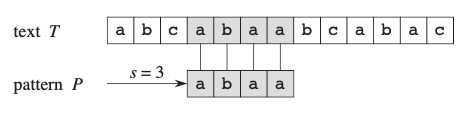
\includegraphics[width = 0.7 \textwidth]{Figure 2.1}
                \caption{An example of the string-matching problem.
                         Given the text $T = abcabaabcabac$ and the pattern $P = abaa$, we want to find all the occurrences of $P$ in $T$.
                         The pattern occurs only once in $T$, starting at shift $s = 3$.}
                \label{fig:example}
            \end{figure}

            \[
                \left\{
                \begin{aligned}
                    & 0 \leq s \leq n - m \\
                    & T[s+1..s+m] = P[1..m] \\
                    & T[s+j] = P[j] \text{ for } (1 \leq j \leq m) \\
                \end{aligned}
                \right.
            \]

        \subsection{Practical application} \label{subsec:practical_application}

            String matching algorithms have many practical applications in different fields:
            \begin{itemize}
                \item Text search: Find the occurrences of words or phrases within documents or long texts.
                \item Natural language processing: Analysing text to recognise language patterns, lexical analysis and parsing of texts.
                \item Computational biology: Analysing DNA, RNA and protein sequences to identify biological patterns and correlations.
                \item Log and structured text analysis: Recognise patterns in large datasets, such as system logs, sensor records, etc.
                \item Data filtering and analysis: They allow information to be extracted from large volumes of structured and unstructured data.
                \item Search engines: Working behind the scenes to identify the most relevant matches between user search queries and content.
                \item Data compression: Used in compression algorithms to find and replace repeated patterns.
                \item Computer security: Identify signatures and patterns of attacks by detecting byte sequences or malicious behaviour in data.
            \end{itemize}

    \newpage

    % The naive string-matching algorithm
    \section{The naive string-matching algorithm} \label{sec:naive_string_matching_algorithm}

        The naive algorithm finds all valid shifts using a loop that checks the condition $P[1..m] = T[s+1..s+m]$ for each of the $n - m + 1$ values of $s$.

        \subsection{Description} \label{subsec:naive_description}

            The naive string-matching algorithm proceeds sliding a ``template'' containing the pattern over the text, noting for which shifts
            all of the characters in the template match the corresponding characters in the text. \\
            The for loop consider each possible shift explicitly, and the if-condition implicitly loops to check corresponding characters
            position until all position match successfully or until a mismatch is found.

        \subsection{Pseudocode} \label{subsec:naive_pseudocode}

            % Naive algorithm pseudocode
            \SetAlgorithmName{}{naive_string_matching_algorithm}{}
            \begin{algorithm}[H] \label{alg:naive_string_matching_algorithm}
                \SetAlgoLined
                \KwData{Text $T$ of size $n$ and pattern $P$ of size $m$}
                \KwResult{All valid shifts with which $P$ occurs in $T$}
                \vspace{0.5em}
                \captionabove{\underline{NAIVE-STRING-MATCHER(T,P)}} \\
                \vspace{0.5em}

                    $n$ \leftarrow T.length\; \\
                    $m$ \leftarrow P.length\; \\
                    \For{$s \leftarrow 0$ \KwTo $n - m$}{
                        \If{$P[1..m] = T[s+1..s+m]$}{
                            print "Pattern occurs with shift" $s$\;
                        }
                    }

            \end{algorithm}

        \subsection{Time complexity} \label{subsec:naive_time_complexity}

            To analyse the time complexity of the algorithm, we can study separately the case in which the pattern occurs only once within the text and the case in which it occurs several times. \\
            In the first case we can identify three situations: the case in which the pattern is at the beginning of the text (best-case),
            the case in which it is at the end of the text (worst-case) and the case in which it is anywhere else in the text (average-case).

            \begin{itemize}
                \item \textbf{Best-case:} the pattern is found immediately at the beginning of the text. In this case the complexity is $\Theta(m)$, where $m$ is the length of the pattern.
                \item \textbf{Worst-case:} the pattern is found at the end of the text. In this case the complexity is $\Theta((n - m + 1)m)$, where $n$ is the length of the text and $m$ is the length of the pattern.
                \item \textbf{Average-case:} the pattern is found anywhere else in the text. In this case the complexity is $O((n - m + 1)m)$, where $n$ is the length of the text and $m$ is the length of the pattern.
            \end{itemize}

            \noindent In the second case, on the other hand, we find only a single case, since the algorithm is forced to view the entire text anyway
            (this is similar to the worst-case treated in the previous situation). In fact, in this case the complexity is $\Theta((n - m + 1)m)$. \\

    % String matching with finite automata
    \section{String matching with finite automata} \label{sec:string_matching_with_finite_automata}

        Some algorithms, in order to reduce the time complexity of the matching process, use a finite automaton to implement a \textbf{preprocessing function} that examines the pattern $P$. \\
        There's in fact a pattern matching technique, the \textbf{string matching with finite automata}, that employs finite automata to efficiently search for occurrences of a given pattern within a larger text.
        These string-matching automata examine each text character exactly once, taking constant time per text character.
        The matching time used, after preprocessing the pattern to build the automaton, is therefore $\Theta(n)$, where $n$ is the length of the text.
        Although it is independent of the size of the text, the time to build the automaton can be large if $\Sigma$ is large.
        In fact, the time to process the pattern using the function $\delta$ is $O(m\lvert\Sigma\rvert)$, where $m$ is the length of the pattern and $\lvert\Sigma\rvert$ is the size of the alphabet. \\

        \subsection{Finite automaton} \label{subsec:finite_automaton}

            \noindent \textbf{Concept:}
            \begin{itemize}
                \item A finite automaton is a simple machine for processing information, used to recognize patterns within input sequences.
                \item It's a computational model consisting of a finite set of states and transitions between those states based on input symbols.
                \item The transition function $\delta$ defines the ways in which one goes from one state to another.
                \item In this context, it's used to recognize whether the pattern occurs in the text.
            \end{itemize}

            \noindent \textbf{Process:}
            \begin{itemize}
                \item Preprocessing: construct a finite automaton that represents the pattern to be matched.
                \item Matching: use the finite automaton to scan through the text and identify potential matches.
            \end{itemize}

            \noindent \textbf{Advantages:}
            \begin{itemize}
                \item Efficient for multiple searches of the same pattern within different texts.
                \item Requires preprocessing only for the pattern.
            \end{itemize}

            \noindent \textbf{Implementation:}
            \begin{itemize}
                \item Construction of Finite Automaton: this involves building a transition function $\delta$ that defines the behavior of the automaton when reading characters of the pattern.
                \item Matching: traverse the text while updating the automaton's state based on the characters encountered. If the automaton reaches an accepting state, a match is found.
            \end{itemize}


    % The Knuth-Morris-Pratt algorithm
    \section{Knuth-Morris-Pratt algorithm} \label{sec:knuth_morris_pratt_algorithm}

        The Knuth-Morris-Pratt algorithm is a string-matching algorithm that uses finite automata to perform string matching.
        In fact, the Knuth-Morris-Pratt algorithm improves the running time of the naive algorithm by using information about the pattern itself to avoid some comparisons, using a preprocessing function \textbf{$\pi$}. \\
        The key idea is that when a mismatch occurs, the pattern itself contains enough information to determine where the next match could begin, thus bypassing re-examination of previously matched characters.

        \subsection{Description}\label{subsec:kmp_description}

             It preprocesses the pattern to create a ``failure function'' that determines potential shifts in case of mismatches during pattern matching.
             This information allows the algorithm to skip unnecessary comparisons, enabling faster pattern identification within the text.
             The KMP algorithm scans the text, leveraging the failure function to avoid redundant checks, and reports all positions where the pattern is found within the text.

        \subsection{Pseudocode} \label{subsec:kmp_pseudocode}

            % KMP algorithm pseudocode
            \SetAlgorithmName{}{kmp_string_matching_algorithm}{}
            \begin{algorithm}[H] \label{alg:kmp_string_matching_algorithm}
                \SetAlgoLined
                \KwData{Text $T$ of size $n$ and pattern $P$ of size $m$}
                \KwResult{All valid shifts with which $P$ occurs in $T$}
                \vspace{0.5em}
                \captionabove{\underline{KMP-MATCHER(T,P)}} \\
                \vspace{0.5em}

                    $n$ \leftarrow T.length\; \\
                    $m$ \leftarrow P.length\; \\
                    \pi \leftarrow \text{COMPUTE-PREFIX-FUNCTION(P)}\; \\
                    $q$ \leftarrow $0$\; \\
                    \For{$i \leftarrow 1$ \KwTo $n$}{
                        \While{$q > 0$ and $P[q+1] \neq T[i]$}{
                            $q \leftarrow \pi[q]$\;
                        }
                        \If{$P[q+1] = T[i]$}{
                            $q \leftarrow q + 1$\;
                        }
                        \If{$q = m$}{
                            print "Pattern occurs with shift" $i - m$\;
                            $q \leftarrow \pi[q]$\;
                        }
                    }

            \end{algorithm}

            \vspace{0.0em}

            % Compute prefix function pseudocode
            \SetAlgorithmName{}{kmp_string_matching_algorithm}{}
            \begin{algorithm}[H] \label{alg:compute_prefix_function}
                \SetAlgoLined
                \KwData{Pattern $P$ of size $m$}
                \KwResult{Prefix function $\pi$}
                \vspace{0.5em}
                \captionabove{\underline{COMPUTE-PREFIX-FUNCTION(P)}} \\
                \vspace{0.5em}

                    $m$ \leftarrow P.length\; \\
                    let $\pi[1..m]$ be a new array\; \\
                    $\pi[1] \leftarrow 0$\; \\
                    $k \leftarrow 0$\; \\
                    \For{$q \leftarrow 2$ \KwTo $m$}{
                        \While{$k > 0$ and $P[k+1] \neq P[q]$}{
                            $k \leftarrow \pi[k]$\;
                        }
                        \If{$P[k+1] = P[q]$}{
                            $k \leftarrow k + 1$\;
                        }
                        $\pi[q] \leftarrow k$\;
                    }
                    \Return $\pi$\;

            \end{algorithm}

        \subsection{Time complexity} \label{subsec:kmp_time_complexity}

            Let us analyse the time complexity of the KMP algorithm by examining the preprocessing and matching phases separately. \\

            \noindent We know that KMP uses a preprocessing function $\pi$, based on the concept of finite automata,
            but implements it in such a way as to be able to compute the transition function $\delta$ efficiently (``on the fly'' as needed).
            In fact, since $\pi[1..m]$ is the array in which the values of the function of the same name are saved, and since $\pi[1..m]$ has only $m$ entries,
            this allows the KMP to save a factor of $\lvert\Sigma\rvert$ in the preprocessing time.
            The time complexity of the preprocessing function $\pi$ of the KMP is therefore $\Theta(m)$.

            The time for the matching phase is therefore $\Theta(n)$, as already mentioned in the Section 4 (String matching with finite automata).
            This is because the preprocessing function allows the algorithm to scroll through the text by examining the characters only once,
            and consequently the complexity is reduced only to the text size, which is $n$.

    \newpage

    % Differences between naive string-matching and KMP algorithms
    \section{Differences between naive string-matching and KMP algorithms} \label{sec:naive_kmp_differences}

        \subsection{Preprocessing} \label{subsec:preprocessing}

            \begin{table}[H]
                \centering
                \begin{tabular}{|c|c|}
                    \hline
                    \textbf{Algorithm} & \textbf{Preprocessing time} \\
                    \hline
                    Naive & {$0$} \\
                    \hline
                    KMP & {$\Theta(m)$} \\
                    \hline
                    \end{tabular}
                \caption{Preprocessing time complexity.}
                \label{tab:preprocessing_time_complexity}
            \end{table}

        \subsection{Matching time complexity} \label{subsec:naive_kmp_time_complexity}

            \quad \textbf{Pattern with only one occurrence in the text:}

            \begin{table}[H]
                \centering
                    \begin{tabular}{|c|c|c|c|}
                        \hhline{~|---|}
                        \multicolumn{1}{c|}{}& \multicolumn{3}{c|}{\textbf{Matching time}} \\
                        \hline
                        \textbf{Algorithm} & \textbf{Best-case} & \textbf{Worst-case} & \textbf{Average-case} \\
                        \hline
                        Naive & $\Theta(m)$ & $\Theta((n-m+1)m)$ & $O((n-m+1)m)$ \\
                        \hline
                        KMP & $\Theta(m)$ & $\Theta(n)$ & $O(n)$ \\
                        \hline
                    \end{tabular}
                \caption{Matching time complexity (case 1).}
                \label{tab:matching_time_complexity_1}
            \end{table}


            \noindent \quad \textbf{Pattern with multiple occurrences in the text:}

            \begin{table}[H]
                \centering
                \begin{tabular}{|c|c|}
                    \hline
                    \textbf{Algorithm} & \textbf{Matching time} \\
                    \hline
                    Naive & $\Theta((n-m+1)m)$ \\
                    \hline
                    KMP & $\Theta(n)$ \\
                    \hline
                \end{tabular}
                \caption{Matching time complexity (case 2).}
                \label{tab:matching_time_complexity_2}
            \end{table}

    % Tests and results
    \section{Tests and results} \label{sec:tests_and_results}

        Various types of tests were generated to analyse the two algorithms, more precisely 4 types of tests:
        random tests (tests with different texts and different patterns),
        tests with the same text of different sizes but same pattern in every test case,
        tests with the same text but different patterns,
        tests with an entire chapter of a book as text and a word as pattern.

        \subsection{Expected performances} \label{subsec:expected_performances}

            Based on the study of the complexities of the two algorithms (\hyperref[sec:naive_kmp_differences]{Section 6}), we can expect them to perform similarly in test cases with small pattern sizes;
            this is because the time for the preprocessing phase of the KMP (which is $\Theta(m)$) tends to that of the naive (which is $0$),
            while the matching time of the naive (which is $\Theta((n-m+1)m)$) tends to that of the KMP (which is $\Theta(n)$).
            We can also guess that, for the same pattern size, as the text size increases,
            the time of the matching phase of the naive increases more than that of the KMP, obviously due to their time complexity.
            Finally, we can expect the KMP to perform better than the naive in test cases with large pattern sizes.

        \subsection{Results} \label{subsec:results}

            Now follows the tests performed.
            Input data and runtimes are shown, the representation of which is provided both in graphical and tabular form.

            \subsubsection{Random tests} \label{subsubsec:tests_1}

                \begin{table}[H]
                    \centering
                        \begin{tabularx}{\textwidth}{|c|X|c|X|c|}
                            \hline
                            \textbf{Test case} & \textbf{Text} & \textbf{n} & \textbf{Pattern} & \textbf{m} \\
                            \hline
                            1 & "abcdefg" & 7 & "cd" & 2 \\
                            \hline
                            2 & "xyxyxy" & 6 & "xy" & 2 \\
                            \hline
                            3 & "bababababa" & 10 & "aba" & 3 \\
                            \hline
                            4 & "racecar" & 7 & "race" & 4 \\
                            \hline
                            5 & "moonlight" & 9 & "light" & 5 \\
                            \hline
                            6 & "patternpattern" & 14 & "pattern" & 7 \\
                            \hline
                            7 & "0123456789012345" & 16 & "2345" & 4 \\
                            \hline
                            8 & "treefrogstreefrogs" & 18 & "treefrogs" & 9 \\
                            \hline
                            9 & "abcdeedcba" & 10 & "deed" & 4 \\
                            \hline
                            10 & "thisisaverylongtextwith nopattern" & 32 & "pattern" & 7 \\
                            \hline
                            11 & "abcdefabcdef" & 12 & "abcdef" & 6 \\
                            \hline
                            12 & "ababababababababababab" & 22 & "abab" & 4 \\
                            \hline
                            13 & "abcdefghi" & 9 & "ijk" & 3 \\
                            \hline
                            14 & "pythonisfun" & 11 & "is" & 2 \\
                            \hline
                            15 & "" & 0 & "pattern" & 7 \\
                            \hline
                            16 & "z" * 100 & 100 & "z" * 10 & 10 \\
                            \hline
                            17 & "abcdefghijklmnopqrstuwxyz" & 25 & "aeiou" & 5 \\
                            \hline
                            18 & "124578915" & 9 & "69" & 2 \\
                            \hline
                            19 & "one" & 3 & "two" & 3 \\
                            \hline
                            20 & "loremipsumdolorsitamet" & 22 & "ipsumdolor" & 10 \\
                            \hline
                        \end{tabularx}
                    \caption{input values in test 1\_1}
                    \label{tab:test_1_1}
                \end{table}

                \newpage

                \begin{table}[H]
                    \centering
                        \begin{tabularx}{\textwidth}{|c|X|c|X|c|}
                            \hline
                            \textbf{Test case} & \textbf{Text} & \textbf{n} & \textbf{Pattern} & \textbf{m} \\
                            \hline
                            1 & "patternabacabac" & 15 & "pattern" & 7 \\
                            \hline
                            2 & "abacabacpattern" & 15 & "pattern" & 7 \\
                            \hline
                            3 & "abacababacabacababacab" & 22 & "abacab" & 6 \\
                            \hline
                            4 & "abababababababababab abababababab" & 32 & "abababababab" & 12 \\
                            \hline
                            5 & "a" * 1000000 + "b" * 5000 & 1005000 & "b" * 5000 & 5000 \\
                            \hline
                            6 & "a" * 1000000 + "ab" * 25000 + "a" * 1000000 & 2050000 & "ab" * 25000 & 50000 \\
                            \hline
                            7 & "ab" * 1000000 & 2000000 & "abab" & 4 \\
                            \hline
                            8 & "abcdefghijklmnopqrstu vwxyz" & 26 & "12345" & 5 \\
                            \hline
                            9 & "abcabcabcabcabc" & 15 & "abc" & 3 \\
                            \hline
                            10 & "abcdefghijklmnopqrstu wxyz" * 20000 & 500000 & "pqrs" * 5000 + "uvwxyz" * 5000 & 50000 \\
                            \hline
                            11 & "0101010101" * 100000 & 1000000 & "01" * 50000 & 100000 \\
                            \hline
                            12 & "abcdefgh" * 50000 & 400000 & "abcd" * 25000 & 100000 \\
                            \hline
                            13 & "a1b2c3d4e5f6g7h8i9j0" * 5000 & 100000 & "12345" * 1000 + "j0" * 1000 & 7000 \\
                            \hline
                            14 & "!@#\$\%\^\&*()\_+=" * 25000 & 325000 & "!@#\$" * 5000 & 20000 \\
                            \hline
                            15 & "abcdefgh" * 100000 &800000  & "abcdefgh" * 50000 & 400000 \\
                            \hline
                            16 & "0123456789" * 200000 & 2000000 & "56789" * 40000 + "23456" * 40000 & 400000 \\
                            \hline
                            17 & "a" * 1000000 + "b" * 5000 & 1005000 & "b" * 5000 & 5000 \\
                            \hline
                            18 & "a" * 1000000 + "ab" * 25000 + "a" * 1000000 & 2050000 & "ab" * 25000 & 50000 \\
                            \hline
                            19 & "ab" * 1000000 & 2000000 & "abab" & 4 \\
                            \hline
                            20 & "a" * 1000000 + "ab" * 25000 + "a" * 1000000 & 2050000 & "ab" * 25000 & 50000 \\
                            \hline
                            21 & "ab" * 1000000 & 2000000 & "abab" & 4 \\
                            \hline
                            22 & "0123456789" * 200000 & 2000000 & "01234" * 40000 & 200000 \\
                            \hline
                            23 & "abcdefghijklmnopqrstu vwxyz" * 50000 & 1300000 & "uvwxyz" * 10000 & 60000 \\
                            \hline
                            24 & "abcdefghijklmnopqrstu wxyz" * 100000 & 2500000 & "pqrs" * 25000 + "uvwxyz" * 25000 & 250000 \\
                            \hline
                            25 & "0101010101" * 50000 & 500000 & "01" * 25000 & 50000 \\
                            \hline
                        \end{tabularx}
                    \caption{input values in test 1\_2}
                    \label{tab:test_1_2}
                \end{table}

                % TEST 1_1

                \newpage

                \begin{figure}[H]
                    \centering
                    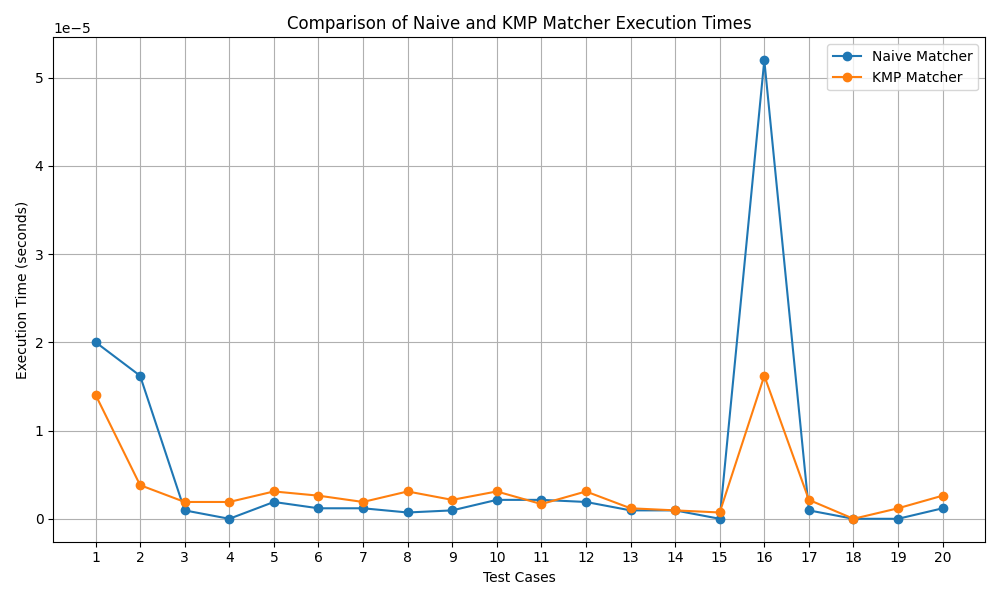
\includegraphics[width = \textwidth]{execution_times_1_1}
                    \caption{chart test 1\_1}
                    \label{fig:chart_test_1_1}
                \end{figure}

                \begin{figure}[H]
                    \centering
                    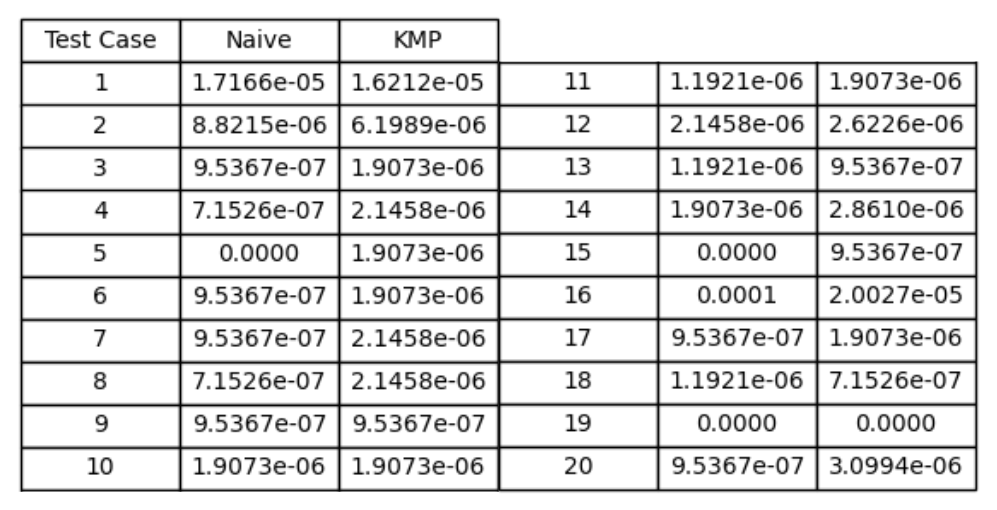
\includegraphics[width = 0.9 \textwidth]{table_execution_times_1_1 (1)}
                    \caption{table test 1\_1}
                    \label{fig:table_test_1_1}
                \end{figure}

                % TEST 1_2

                \newpage

                \begin{figure}[H]
                    \centering
                    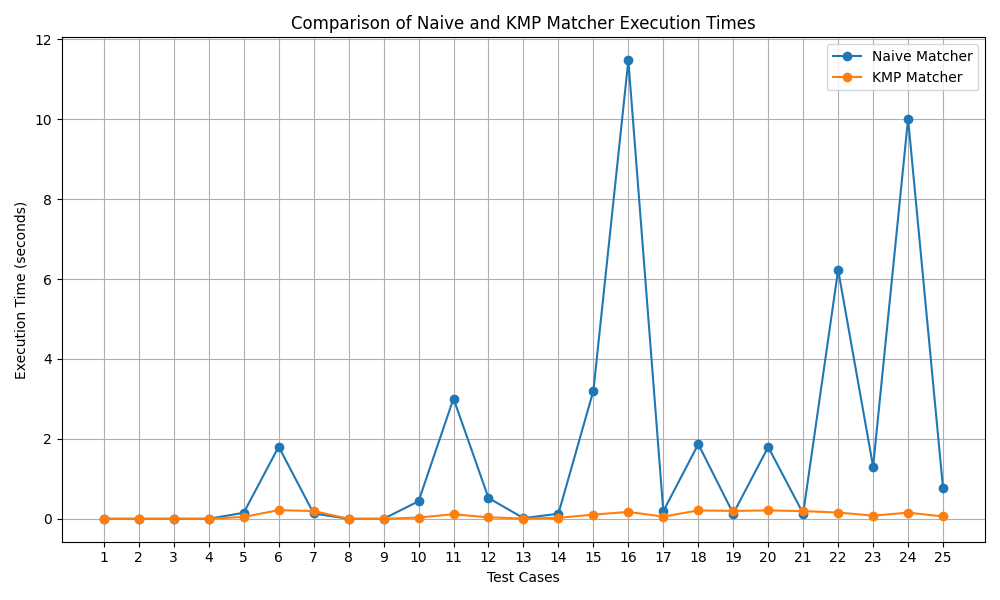
\includegraphics[width = \textwidth]{execution_times_1_2}
                    \caption{chart test 1\_2}
                    \label{fig:chart_test_1_2}
                \end{figure}

                \begin{figure}[H]
                    \centering
                    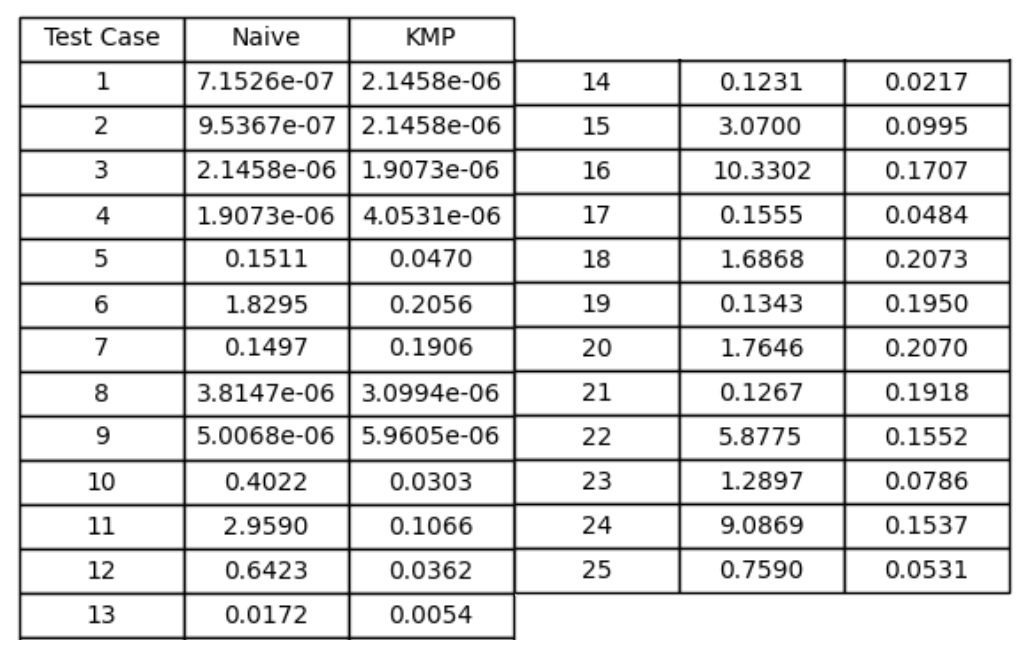
\includegraphics[width = 0.9 \textwidth]{table_execution_times_1_2 (1)}
                    \caption{table test 1\_2}
                    \label{fig:table_test_1_2}
                \end{figure}

            \newpage

            \subsubsection{Tests with the same text of different sizes but same pattern in every test case} \label{subsubsec:tests_2}

                % TEST 2_1

                \begin{table}[!htb]
                        \begin{minipage}{.5\linewidth}
                            \centering
                                \begin{tabular}{ll}
                                    \textbf{Text} & \textbf{n} \\
                                    \hline
                                    "0123456789" * 2000 & 20000 \\
                                    "0123456789" * 20000 & 200000 \\
                                    "0123456789" * 200000 & 2000000 \\
                                    "0123456789" * 2000000 & 20000000 \\
                                    "0123456789" * 20000000 & 200000000 \\
                                \end{tabular}
                        \end{minipage}%
                        \begin{minipage}{.5\linewidth}
                            \centering
                                \begin{tabular}{ll}
                                    \textbf{Pattern} & \textbf{m} \\
                                    \hline
                                    "56789" * 40 + "23456" * 40 & 400 \\
                                    "56789" * 40 + "23456" * 40 & 400 \\
                                    "56789" * 40 + "23456" * 40 & 400 \\
                                    "56789" * 40 + "23456" * 40 & 400 \\
                                    "56789" * 40 + "23456" * 40 & 400 \\
                                \end{tabular}
                        \end{minipage}
                    \label{tab:test_2_1}
                \end{table}

                \begin{figure}[H]
                    \centering
                    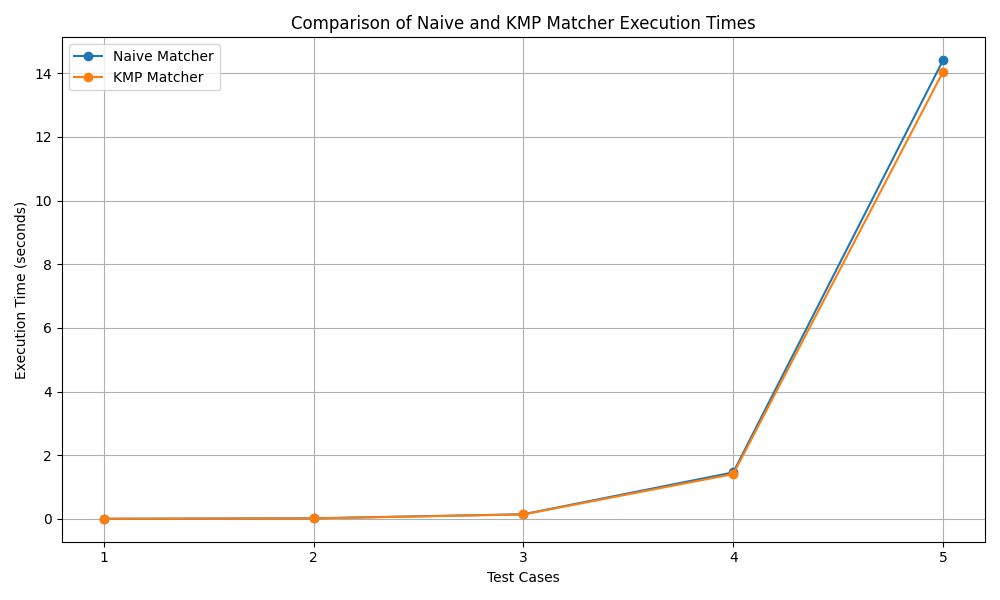
\includegraphics[width = \textwidth]{execution_times_2_1}
                    \caption{chart test 2\_1}
                    \label{fig:chart_test_2_1}
                \end{figure}

                \begin{figure}[H]
                    \centering
                    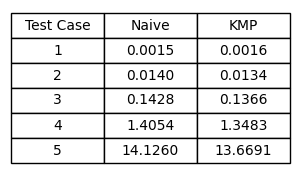
\includegraphics[width = 0.5 \textwidth]{table_execution_times_2_1}
                    \caption{table test 2\_1}
                    \label{fig:table_test_2_1}
                \end{figure}

                \newpage

                % TEST 2_2

                \begin{table}[!htb]
                        \begin{minipage}{.5\linewidth}
                            \centering
                                \begin{tabular}{ll}
                                    \textbf{Text} & \textbf{n} \\
                                    \hline
                                    "0123456789" * 2000 & 20000 \\
                                    "0123456789" * 20000 & 200000 \\
                                    "0123456789" * 200000 & 2000000 \\
                                    "0123456789" * 2000000 & 20000000 \\
                                    "0123456789" * 20000000 & 200000000 \\
                                \end{tabular}
                        \end{minipage}%
                        \begin{minipage}{.5\linewidth}
                            \centering
                                \begin{tabular}{ll}
                                    \textbf{Pattern} & \textbf{m} \\
                                    \hline
                                    "56789" * 400 + "23456" * 400 & 4000 \\
                                    "56789" * 400 + "23456" * 400 & 4000 \\
                                    "56789" * 400 + "23456" * 400 & 4000 \\
                                    "56789" * 400 + "23456" * 400 & 4000 \\
                                    "56789" * 400 + "23456" * 400 & 4000 \\
                                \end{tabular}
                        \end{minipage}
                    \label{tab:test_2_2}
                \end{table}

                \begin{figure}[H]
                    \centering
                    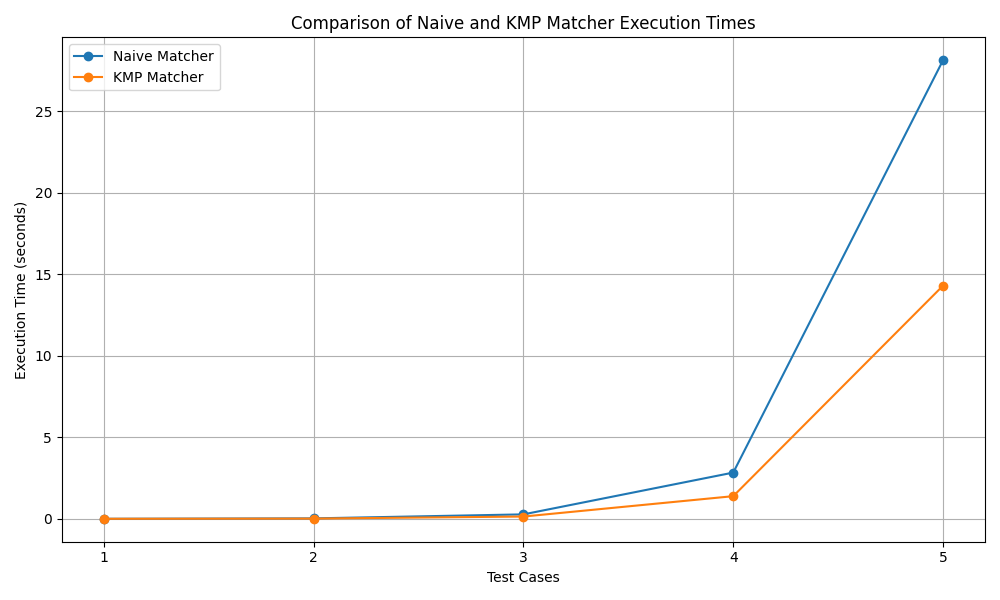
\includegraphics[width = \textwidth]{execution_times_2_2}
                    \caption{chart test 2\_2}
                    \label{fig:chart_test_2_2}
                \end{figure}

                \begin{figure}[H]
                    \centering
                    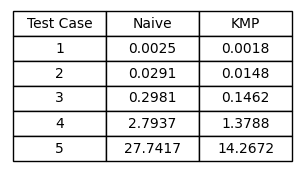
\includegraphics[width = 0.5 \textwidth]{table_execution_times_2_2}
                    \caption{table test 2\_2}
                    \label{fig:table_test_2_2}
                \end{figure}

                \newpage

                % TEST 2_3

                \begin{table}[!htb]
                        \begin{minipage}{.5\linewidth}
                            \centering
                                \begin{tabular}{ll}
                                    \textbf{Text} & \textbf{n} \\
                                    \hline
                                    "0123456789" * 2000 & 20000 \\
                                    "0123456789" * 20000 & 200000 \\
                                    "0123456789" * 200000 & 2000000 \\
                                    "0123456789" * 2000000 & 20000000 \\
                                    "0123456789" * 20000000 & 200000000 \\
                                \end{tabular}
                        \end{minipage}%
                        \begin{minipage}{.5\linewidth}
                            \centering
                                \begin{tabular}{ll}
                                    \textbf{Pattern} & \textbf{m} \\
                                    \hline
                                    "56789" * 4000 + "23456" * 4000 & 40000 \\
                                    "56789" * 4000 + "23456" * 4000 & 40000 \\
                                    "56789" * 4000 + "23456" * 4000 & 40000 \\
                                    "56789" * 4000 + "23456" * 4000 & 40000 \\
                                    "56789" * 4000 + "23456" * 4000 & 40000 \\
                                \end{tabular}
                        \end{minipage}
                    \label{tab:test_2_3}
                \end{table}

                \begin{figure}[H]
                    \centering
                    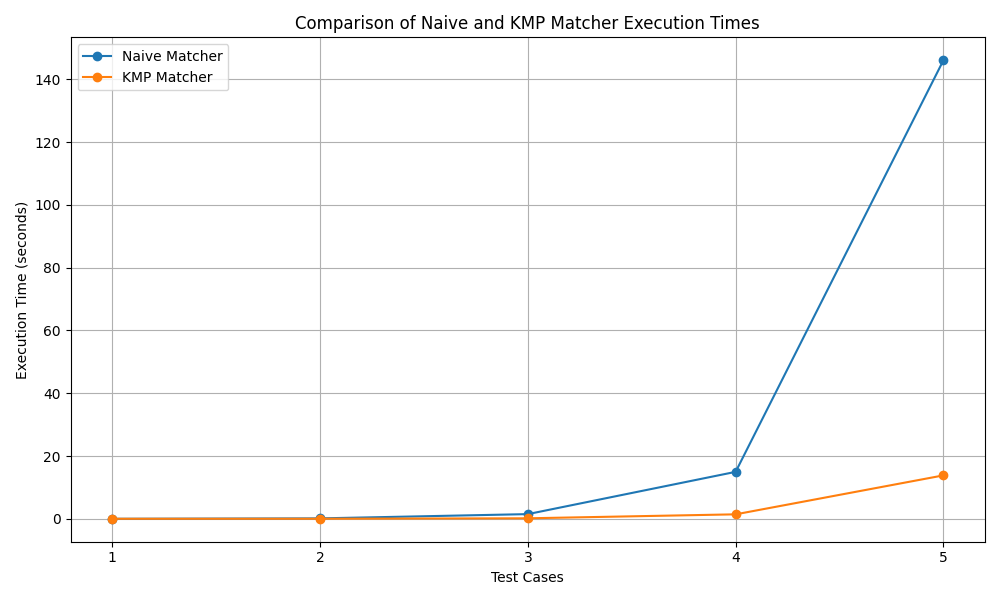
\includegraphics[width = \textwidth]{execution_times_2_3}
                    \caption{chart test 2\_3}
                    \label{fig:chart_test_2_3}
                \end{figure}

                \begin{figure}[H]
                    \centering
                    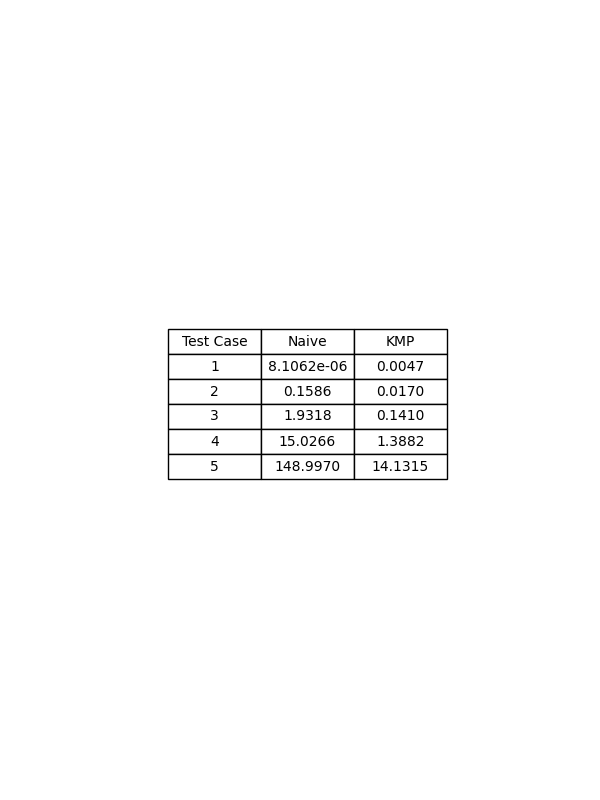
\includegraphics[width = 0.5 \textwidth]{table_execution_times_2_3}
                    \caption{table test 2\_3}
                    \label{fig:table_test_2_3}
                \end{figure}

            \newpage

            \subsubsection{Tests with the same text but different patterns} \label{subsubsec:tests_3}

                % TEST 3_1

                \begin{table}[!htb]
                        \begin{minipage}{.5\linewidth}
                            \centering
                                \begin{tabular}{ll}
                                    \textbf{Text} & \textbf{n} \\
                                    \hline
                                    "0123456789" * 200000000 & 2000000000 \\
                                    "0123456789" * 200000000 & 2000000000 \\
                                    "0123456789" * 200000000 & 2000000000 \\
                                    "0123456789" * 200000000 & 2000000000 \\
                                    "0123456789" * 200000000 & 2000000000 \\
                                \end{tabular}
                        \end{minipage}%
                        \begin{minipage}{.5\linewidth}
                            \centering
                                \begin{tabular}{ll}
                                    \textbf{Pattern} & \textbf{m} \\
                                    \hline
                                    "56789" * 4 + "23456" * 4 & 40 \\
                                    "56789" * 40 + "23456" * 40 & 400 \\
                                    "56789" * 400 + "23456" * 400 & 4000 \\
                                    "56789" * 4000 + "23456" * 4000 & 40000 \\
                                    "56789" * 40000 + "23456" * 40000 & 400000 \\
                                \end{tabular}
                        \end{minipage}
                    \label{tab:test_3_1}
                \end{table}

                \begin{figure}[H]
                    \centering
                    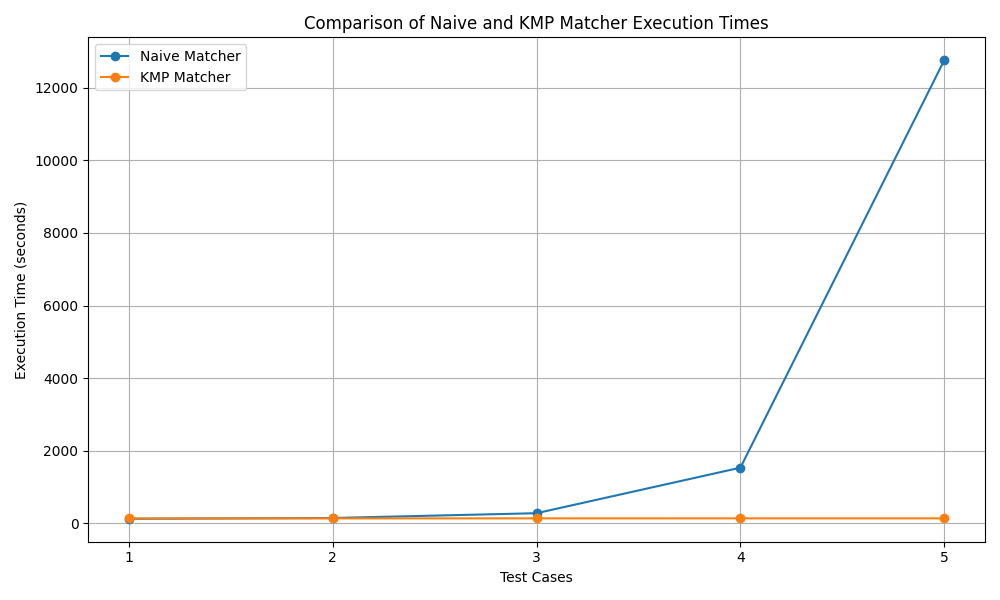
\includegraphics[width = \textwidth]{execution_times_3_1}
                    \caption{chart test 3\_1}
                    \label{fig:chart_test_3_1}
                \end{figure}

                \begin{figure}[H]
                    \centering
                    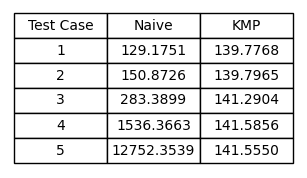
\includegraphics[width = 0.5 \textwidth]{table_execution_times_3_1}
                    \caption{table test 3\_1}
                    \label{fig:table_test_3_1}
                \end{figure}

            \newpage

            \newgeometry{top=2.9cm, bottom=2.8cm}

            \subsubsection{Tests with an entire chapter of a book as text and a word as pattern} \label{subsubsec:tests_4}

                % TEST 4_1

                First chapter of the book ``The Hobbit'' by J.R.R. Tolkien as text and the word ``hobbit'' as pattern.
                \begin{verbatim}(http://hbcsni.org/images/9th_Honors_CP_THE_HOBBIT_textbook.pdf)\end{verbatim}

                \begin{table}[!htb]
                        \begin{minipage}{.5\linewidth}
                            \centering
                                \begin{tabular}{ll}
                                    \textbf{Text} & \textbf{n} \\
                                    \hline
                                    An Unexpected Party & 46211 \\
                                \end{tabular}
                        \end{minipage}%
                        \begin{minipage}{.5\linewidth}
                            \centering
                                \begin{tabular}{ll}
                                    \textbf{Pattern} & \textbf{m} \\
                                    \hline
                                    "hobbit" & 6 \\
                                \end{tabular}
                        \end{minipage}
                    \label{tab:test_4_1}
                \end{table}


                %    \begin{figure}[H]
                %        \centering
                %        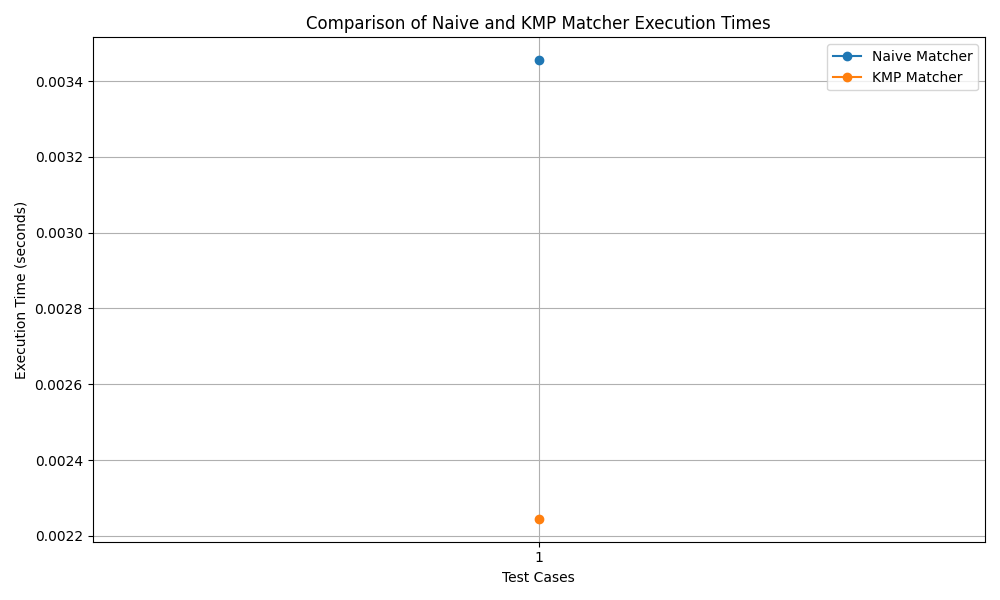
\includegraphics[width = \textwidth]{execution_times_4_1}
                %        \caption{chart test 4\_1}
                %        \label{fig:chart_test_4_1}
                %    \end{figure}


                \begin{figure}[H]
                    \centering
                    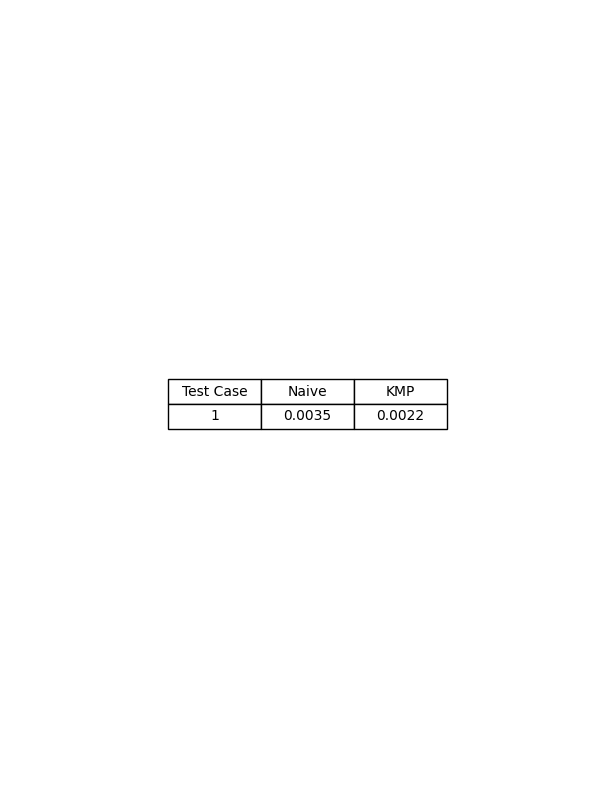
\includegraphics[width = 0.5 \textwidth]{table_execution_times_4_1}
                    \caption{table test 4\_1}
                    \label{fig:table_test_4_1}
                \end{figure}

    %\newpage % to be uncommented if the test 4_1 chart is uncommented -> check even the geometry of the page

    % Conclusions
    \section{Tests discussion and conclusions} \label{sec:conclusions}

        Tests confirm what we expected and each test case gives us information about it. \\
        In the random tests (\hyperref[subsubsec:tests_1]{Section 7.2.1}) we can see, especially by looking at the graphs (\hyperref[fig:chart_test_1_1]{Fig. 2}, \hyperref[fig:chart_test_1_2]{Fig. 4}) that the largest gap between
        the execution times of the two algorithms occurs in the test cases where the pattern size is largest,
        e.g.: in test 1\_1 the test case 20, while in test 1\_2 the test cases 6, 11, 15, 16, 18, 20, 22, 24. \\
        Examining the tests of the second type (\hyperref[subsubsec:tests_2]{Section 7.2.2}), we can note that in the cases in which the size of the pattern is moderately ``small''
        (in the tests carried out we speak of the order of hundreds) there is not much difference between
        the execution times of the naive and the KMP, even as the size of the text increases (the difference remains rather constant,
        especially in the 2\_1 test (\hyperref[fig:chart_test_2_1]{Fig. 6}), where the times seem to overlap). \\
        In fact, in tests 2\_2 and 2\_3 (\hyperref[fig:chart_test_2_2]{Fig. 8}, \hyperref[fig:chart_test_2_3]{Fig. 10}), the gap between the execution times of the two algorithms grows considerably as the size of the text increases
        (in these two tests we speak of a pattern size in the order of thousands in the first test, and in the order of tens of thousands in the second). \\
        The final confirmation is provided by test 3\_1 (\hyperref[subsubsec:tests_3]{Section 7.2.3}) in which we both vary the pattern on the same text with a set size of 200000000,
        going from an m = 40 to an m = 400000. In fact, in this test we see how the times of the naive ``explode'' compared to those of the kmp (\hyperref[fig:chart_test_3_1]{Fig. 12}) . \\
        We then have a ``practice'' test (\hyperref[subsubsec:tests_4]{Section 7.2.4}) in which we test the two algorithms on a chapter of a famous book: the first chapter of ``The Hobbit'' by J.R.R. Tolkien.
        Here too we see how, given a pattern of rather small size, the two times resemble each other (\hyperref[fig:table_test_4_1]{Fig. 14}). \\

        \noindent In conclusion, we can say that the KMP algorithm is more efficient than the naive algorithm in the case of large pattern sizes,
        and offers a very good solution when performing numerous tests with the same pattern as the algorithm allows us to keep the result
        of the COMPUTE-PREFIX-FUNCTION(P) (the preprocessing function \pi \text{ that has complexity } $\Theta(m)$) and to have a matching phase with
        complexity always equal to $\Theta(n)$ where $n$ is the size of the text.

    \restoregeometry

\end{document}